\documentclass[11pt]{article}

\usepackage[margin=1in]{geometry}
\usepackage{graphicx}
\usepackage{array}
\usepackage{longtable}
\usepackage{hyperref}
\usepackage{booktabs}
\usepackage{xcolor}
\usepackage{tikz}
\usepackage{float}
\usepackage{enumitem}
\usepackage{fancyhdr}
\usepackage{titlesec}
\usepackage{tcolorbox}
\usepackage{tabularx}
\usepackage{multirow}
\usepackage{caption}
\usepackage{subcaption}
\usepackage{listings}
\usepackage{makecell}
\usepackage{amssymb}
\usepackage{textcomp}

\usetikzlibrary{shapes.geometric, arrows.meta, positioning, fit, backgrounds, calc, decorations.pathreplacing, shapes.multipart, matrix, shadows}

% Color definitions
\definecolor{interfacecolor}{RGB}{70,130,180}
\definecolor{operationcolor}{RGB}{60,179,113}
\definecolor{eventcolor}{RGB}{255,165,0}
\definecolor{errorcolor}{RGB}{220,53,69}
\definecolor{flowcolor}{RGB}{100,100,100}
\definecolor{sectionblue}{RGB}{31,78,121}
\definecolor{lightgray}{RGB}{245,245,245}
\definecolor{warningred}{RGB}{220,53,69}
\definecolor{successgreen}{RGB}{40,167,69}
\definecolor{infoblue}{RGB}{23,162,184}
\definecolor{providedcolor}{RGB}{40,167,69}
\definecolor{requiredcolor}{RGB}{255,193,7}
\definecolor{synccolor}{RGB}{70,130,180}
\definecolor{asynccolor}{RGB}{186,85,211}
\definecolor{restcolor}{RGB}{97,175,239}
\definecolor{grpccolor}{RGB}{244,180,0}
\definecolor{graphqlcolor}{RGB}{229,53,171}
\definecolor{kafkacolor}{RGB}{35,31,32}
\definecolor{deprecatedcolor}{RGB}{108,117,125}
\definecolor{stablecolor}{RGB}{40,167,69}
\definecolor{betacolor}{RGB}{255,193,7}

% Hyperref setup
\hypersetup{
    colorlinks=true,
    linkcolor=sectionblue,
    urlcolor=sectionblue,
    citecolor=sectionblue
}

% Header and footer
\pagestyle{fancy}
\setlength{\headheight}{14pt}
\addtolength{\topmargin}{-2pt}
\fancyhf{}
\fancyhead[L]{\leftmark}
\fancyhead[R]{Interface Documentation}
\fancyfoot[C]{\thepage}
\renewcommand{\headrulewidth}{0.4pt}
\renewcommand{\footrulewidth}{0.4pt}

% Section formatting
\titleformat{\section}
  {\normalfont\Large\bfseries\color{sectionblue}}{\thesection}{1em}{}
\titleformat{\subsection}
  {\normalfont\large\bfseries\color{sectionblue!80}}{\thesubsection}{1em}{}
\titleformat{\subsubsection}
  {\normalfont\normalsize\bfseries\color{sectionblue!60}}{\thesubsubsection}{1em}{}

% Custom box environments
\newtcolorbox{keypoint}{
    colback=blue!5,
    colframe=sectionblue,
    title=Key Point,
    fonttitle=\bfseries
}

\newtcolorbox{warning}{
    colback=red!5,
    colframe=warningred,
    title=Warning,
    fonttitle=\bfseries
}

\newtcolorbox{bestpractice}{
    colback=green!5,
    colframe=successgreen,
    title=Best Practice,
    fonttitle=\bfseries
}

\newtcolorbox{example}{
    colback=lightgray,
    colframe=flowcolor,
    title=Example,
    fonttitle=\bfseries
}

\newtcolorbox{definition}{
    colback=infoblue!10,
    colframe=infoblue,
    title=Definition,
    fonttitle=\bfseries
}

\newtcolorbox{template}{
    colback=white,
    colframe=flowcolor,
    title=Template,
    fonttitle=\bfseries
}

\newtcolorbox{interfacebox}[1][]{
    colback=interfacecolor!5,
    colframe=interfacecolor,
    title=#1,
    fonttitle=\bfseries,
    breakable
}

\newtcolorbox{operationbox}[1][]{
    colback=operationcolor!5,
    colframe=operationcolor,
    title=#1,
    fonttitle=\bfseries
}

\newtcolorbox{eventbox}[1][]{
    colback=eventcolor!10,
    colframe=eventcolor,
    title=#1,
    fonttitle=\bfseries
}

\tcbuselibrary{listings,breakable,skins}

% Code listing style
\lstdefinestyle{json}{
    basicstyle=\ttfamily\small,
    breaklines=true,
    frame=single,
    backgroundcolor=\color{lightgray},
    keywordstyle=\color{sectionblue},
    stringstyle=\color{operationcolor},
    showstringspaces=false,
    literate=
     *{0}{{{\color{eventcolor}0}}}{1}
      {1}{{{\color{eventcolor}1}}}{1}
      {2}{{{\color{eventcolor}2}}}{1}
      {3}{{{\color{eventcolor}3}}}{1}
      {4}{{{\color{eventcolor}4}}}{1}
      {5}{{{\color{eventcolor}5}}}{1}
      {6}{{{\color{eventcolor}6}}}{1}
      {7}{{{\color{eventcolor}7}}}{1}
      {8}{{{\color{eventcolor}8}}}{1}
      {9}{{{\color{eventcolor}9}}}{1}
}

% YAML language definition for listings (used for OpenAPI/AsyncAPI examples)
\lstdefinelanguage{yaml}{
  sensitive=false,
  morecomment=[l]{\#},
  morestring=[b]",
  morestring=[b]',
  basicstyle=\ttfamily\small
}

\lstdefinestyle{http}{
    basicstyle=\ttfamily\small,
    breaklines=true,
    frame=single,
    backgroundcolor=\color{lightgray},
    moredelim=[is][\color{operationcolor}]{|}{|},
    moredelim=[is][\color{sectionblue}\bfseries]{@}{@}
}

\lstset{
    basicstyle=\ttfamily\small,
    breaklines=true,
    frame=single,
    backgroundcolor=\color{lightgray},
    keywordstyle=\color{sectionblue},
    commentstyle=\color{successgreen},
    stringstyle=\color{eventcolor},
    showstringspaces=false
}

% Custom column types
\newcolumntype{L}[1]{>{\raggedright\arraybackslash}p{#1}}
\newcolumntype{C}[1]{>{\centering\arraybackslash}p{#1}}
\newcolumntype{R}[1]{>{\raggedleft\arraybackslash}p{#1}}

% Status badges
\newcommand{\statusstable}{\textcolor{stablecolor}{\textbf{[STABLE]}}}
\newcommand{\statusbeta}{\textcolor{betacolor}{\textbf{[BETA]}}}
\newcommand{\statusdeprecated}{\textcolor{deprecatedcolor}{\textbf{[DEPRECATED]}}}
\newcommand{\statusdraft}{\textcolor{infoblue}{\textbf{[DRAFT]}}}

% HTTP method badges
\newcommand{\httpget}{\colorbox{operationcolor!80}{\textcolor{white}{\textbf{\small GET}}}}
\newcommand{\httppost}{\colorbox{eventcolor!80}{\textcolor{white}{\textbf{\small POST}}}}
\newcommand{\httpput}{\colorbox{interfacecolor!80}{\textcolor{white}{\textbf{\small PUT}}}}
\newcommand{\httppatch}{\colorbox{asynccolor!80}{\textcolor{white}{\textbf{\small PATCH}}}}
\newcommand{\httpdelete}{\colorbox{errorcolor!80}{\textcolor{white}{\textbf{\small DELETE}}}}

\title{%
    \vspace{-1cm}
    \textbf{\Huge Software Architecture Documentation}\\[12pt]
    \Large Interface Documentation\\[8pt]
    \large A Comprehensive Guide to Documenting APIs, Events,\\
    Protocols, and System Boundaries
}
\author{%
    \textit{Architecture Documentation Series}\\[4pt]
    \small Based on OpenAPI, AsyncAPI, IEEE Standards, and Industry Best Practices
}
\date{\today}

\begin{document}

\maketitle
\thispagestyle{empty}

\vspace{0.8cm}

\begin{abstract}
\noindent
Interface documentation describes the contracts through which architectural elements interact---the APIs, events, protocols, and data formats that define system boundaries. Well-documented interfaces enable independent development, testing, and evolution of system components while ensuring interoperability and maintainability. This comprehensive guide establishes principles and practices for documenting all types of interfaces: REST APIs, GraphQL endpoints, gRPC services, message queues, event streams, file formats, and hardware protocols. The document covers interface taxonomy, operation specifications, data schemas, protocol details, error handling, quality of service, security requirements, versioning strategies, and governance processes. Whether designing public APIs, internal service contracts, or integration interfaces, this guide provides the foundation for clear, complete, and consumable interface documentation.
\end{abstract}

\vfill

\begin{center}
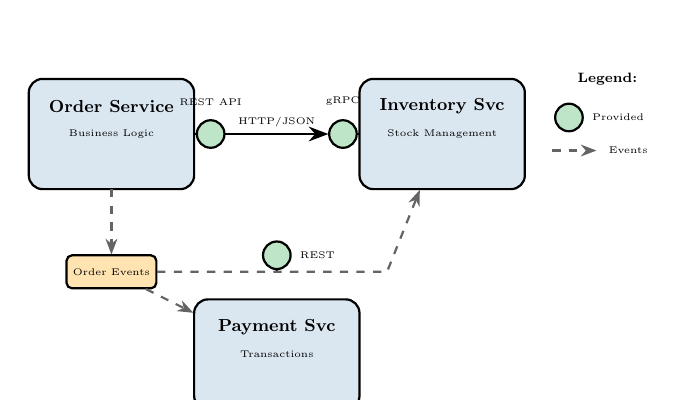
\begin{tikzpicture}[
    scale=0.7,
    transform shape,
    service/.style={draw, thick, fill=interfacecolor!20, minimum width=3cm, minimum height=2cm, rounded corners=5pt},
    interface/.style={draw, thick, fill=white, minimum width=0.8cm, minimum height=0.5cm, font=\tiny},
    provided/.style={draw, thick, fill=providedcolor!30, circle, minimum size=0.5cm},
    required/.style={draw, thick, fill=requiredcolor!30, semicircle, minimum size=0.5cm},
    arrow/.style={-{Stealth[length=2.5mm]}, thick},
    data/.style={-{Stealth[length=2mm]}, thick, dashed, flowcolor}
]
    % Services
    \node[service] (orderSvc) at (0,0) {};
    \node[font=\small\bfseries] at (0,0.5) {Order Service};
    \node[font=\tiny] at (0,0) {Business Logic};
    
    \node[service] (invSvc) at (6,0) {};
    \node[font=\small\bfseries] at (6,0.5) {Inventory Svc};
    \node[font=\tiny] at (6,0) {Stock Management};
    
    \node[service] (paySvc) at (3,-4) {};
    \node[font=\small\bfseries] at (3,-3.5) {Payment Svc};
    \node[font=\tiny] at (3,-4) {Transactions};
    
    % Provided interfaces (lollipops)
    \node[provided] (orderApi) at (1.8,0) {};
    \node[font=\tiny, above] at (1.8,0.4) {REST API};
    \draw[thick] (1.5,0) -- (orderApi);
    
    \node[provided] (invApi) at (4.2,0) {};
    \node[font=\tiny, above] at (4.2,0.4) {gRPC};
    \draw[thick] (4.5,0) -- (invApi);
    
    \node[provided] (payApi) at (3,-2.2) {};
    \node[font=\tiny, right] at (3.3,-2.2) {REST};
    \draw[thick] (3,-2.5) -- (payApi);
    
    % Event interfaces
    \node[draw, thick, fill=eventcolor!30, minimum width=1.5cm, minimum height=0.6cm, rounded corners=2pt, font=\tiny] (events) at (0,-2.5) {Order Events};
    \draw[data] (0,-1) -- (events);
    \draw[data] (events) -- (paySvc);
    \draw[data] (events) -| (5,-2.5) -- (invSvc);
    
    % Connections
    \draw[arrow] (orderApi) -- node[above, font=\tiny] {HTTP/JSON} (invApi);
    
    % Legend
    \node[font=\scriptsize\bfseries] at (9,1) {Legend:};
    \node[provided] at (8.3,0.3) {};
    \node[font=\tiny, right] at (8.6,0.3) {Provided};
    \draw[data] (8,-.3) -- (8.8,-0.3);
    \node[font=\tiny, right] at (8.9,-0.3) {Events};
\end{tikzpicture}
\end{center}

\newpage
\tableofcontents
\newpage

%==============================================================================
\section{Introduction to Interface Documentation}
%==============================================================================

\subsection{Definition and Purpose}

An interface is a boundary across which two architectural elements interact. Interface documentation describes what consumers need to know to successfully use an interface---the operations available, data formats expected, protocols used, and behaviors guaranteed.

\begin{definition}
\textbf{Interface Documentation} is the specification of the externally visible properties of an architectural element's boundary---the contract that defines how other elements can interact with it, including the syntax (operations, data types), semantics (behavior, constraints), and pragmatics (protocols, quality attributes) of that interaction.
\end{definition}

Interface documentation serves several critical purposes. First, it enables \textbf{independent development} by allowing teams to build consumers and providers in parallel based on agreed contracts. Second, it supports \textbf{integration testing} by providing the specification against which implementations are validated. Third, it facilitates \textbf{evolution} by making change impact analysis possible through explicit contract versioning. Fourth, it enables \textbf{discovery} by helping developers find and understand available capabilities. Fifth, it ensures \textbf{interoperability} by precisely defining exchange formats and protocols.

\subsection{The Cost of Poor Interface Documentation}

\begin{warning}
\textbf{Consequences of Inadequate Interface Documentation:}

\textbf{Integration failures:} Teams discover incompatibilities late in development when integration is attempted, causing delays and rework.

\textbf{Breaking changes:} Without clear contracts, changes inadvertently break consumers, causing production incidents.

\textbf{Duplicate implementations:} Teams build redundant services because they cannot discover existing capabilities.

\textbf{Support burden:} Interface owners spend excessive time answering questions that documentation should address.

\textbf{Security vulnerabilities:} Unclear authentication and authorization requirements lead to inconsistent security implementations.

\textbf{Performance problems:} Undocumented rate limits and quotas cause cascading failures under load.
\end{warning}

\subsection{Interface Documentation in Context}

Interface documentation complements the Element Catalog by providing detailed specifications for how elements interact. While the catalog describes what an element is and does, interface documentation describes how to interact with it.

\begin{figure}[H]
\centering
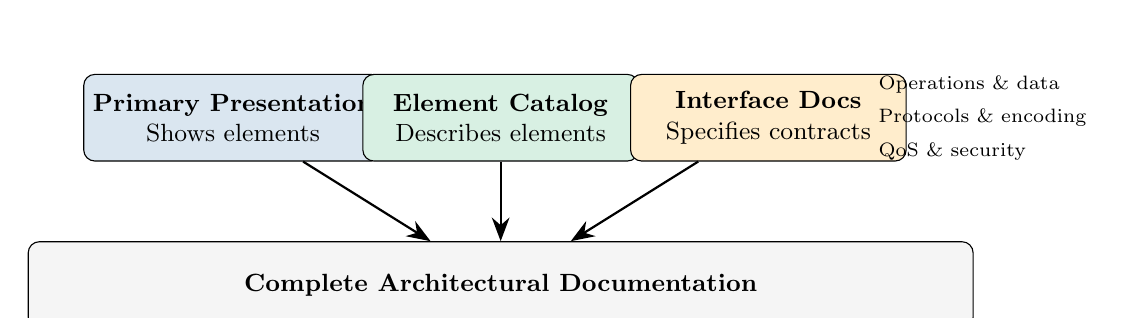
\begin{tikzpicture}[
    scale=0.85,
    box/.style={draw, rounded corners, minimum width=3.5cm, minimum height=1.1cm, align=center, font=\small},
    arrow/.style={-{Stealth[length=3mm]}, thick}
]
    % Documentation components
    \node[box, fill=interfacecolor!20] (primary) at (-4,2) {\textbf{Primary Presentation}\\Shows elements};
    \node[box, fill=operationcolor!20] (catalog) at (0,2) {\textbf{Element Catalog}\\Describes elements};
    \node[box, fill=eventcolor!20] (interface) at (4,2) {\textbf{Interface Docs}\\Specifies contracts};
    
    % Complete view
    \node[box, fill=lightgray, minimum width=12cm] (view) at (0,-0.5) {\textbf{Complete Architectural Documentation}};
    
    % Arrows
    \draw[arrow] (primary) -- (view);
    \draw[arrow] (catalog) -- (view);
    \draw[arrow] (interface) -- (view);
    
    % Questions answered
    \node[font=\scriptsize, right] at (5.5,2.5) {Operations \& data};
    \node[font=\scriptsize, right] at (5.5,2) {Protocols \& encoding};
    \node[font=\scriptsize, right] at (5.5,1.5) {QoS \& security};
\end{tikzpicture}
\caption{Interface Documentation within Architecture Documentation}
\end{figure}

\subsection{Standards and Specifications}

Interface documentation builds on established standards. OpenAPI (formerly Swagger) provides the specification for REST API documentation. AsyncAPI extends similar concepts to event-driven interfaces. gRPC/Protocol Buffers define service interfaces for RPC. GraphQL Schema Definition Language specifies GraphQL APIs. WSDL documents SOAP web services. IEEE 830 and ISO/IEC/IEEE 29148 provide general requirements specification guidance.

%==============================================================================
\section{Interface Taxonomy}
%==============================================================================

\subsection{Interface Classification}

Interfaces can be classified along several dimensions to guide documentation approach and depth.

\subsubsection{By Direction}

\begin{longtable}{@{}L{2.5cm} L{4.5cm} L{5.5cm}@{}}
\caption{Interface Classification by Direction} \\
\toprule
\textbf{Direction} & \textbf{Description} & \textbf{Examples} \\
\midrule
\endfirsthead
\toprule
\textbf{Direction} & \textbf{Description} & \textbf{Examples} \\
\midrule
\endhead
\bottomrule
\endlastfoot
Provided & Interface offered by element for others to consume & REST API; gRPC service; event publisher \\
Required & Interface that element needs from others & Database connection; external API client \\
Bidirectional & Two-way communication channel & WebSocket; message queue with reply \\
\end{longtable}

\subsubsection{By Interaction Pattern}

\begin{longtable}{@{}L{3cm} L{4cm} L{5.5cm}@{}}
\caption{Interface Classification by Interaction Pattern} \\
\toprule
\textbf{Pattern} & \textbf{Characteristics} & \textbf{Technologies} \\
\midrule
\endfirsthead
\toprule
\textbf{Pattern} & \textbf{Characteristics} & \textbf{Technologies} \\
\midrule
\endhead
\bottomrule
\endlastfoot
Request-Response & Synchronous; caller waits for result & REST, gRPC, GraphQL \\
Fire-and-Forget & Asynchronous; no response expected & Message queue publish \\
Publish-Subscribe & One-to-many event distribution & Kafka, RabbitMQ, SNS \\
Streaming & Continuous data flow & gRPC streaming, WebSocket, SSE \\
Callback/Webhook & Asynchronous notification to caller & HTTP webhooks \\
Polling & Consumer periodically checks for updates & REST polling, long-polling \\
\end{longtable}

\subsubsection{By Technology}

\begin{figure}[H]
\centering
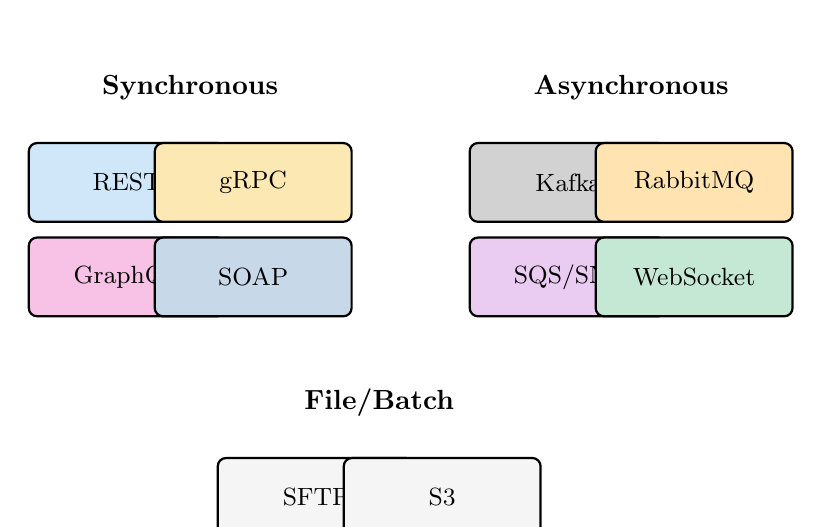
\begin{tikzpicture}[
    scale=0.8,
    tech/.style={draw, thick, minimum width=2.5cm, minimum height=1cm, rounded corners=3pt, font=\small, align=center}
]
    % Synchronous
    \node[font=\bfseries] at (-4,3) {Synchronous};
    \node[tech, fill=restcolor!30] (rest) at (-5,1.5) {REST};
    \node[tech, fill=grpccolor!30] (grpc) at (-3,1.5) {gRPC};
    \node[tech, fill=graphqlcolor!30] (gql) at (-5,0) {GraphQL};
    \node[tech, fill=interfacecolor!30] (soap) at (-3,0) {SOAP};
    
    % Asynchronous
    \node[font=\bfseries] at (3,3) {Asynchronous};
    \node[tech, fill=kafkacolor!20] (kafka) at (2,1.5) {Kafka};
    \node[tech, fill=eventcolor!30] (rabbit) at (4,1.5) {RabbitMQ};
    \node[tech, fill=asynccolor!30] (sqs) at (2,0) {SQS/SNS};
    \node[tech, fill=operationcolor!30] (ws) at (4,0) {WebSocket};
    
    % File/Batch
    \node[font=\bfseries] at (-1,-2) {File/Batch};
    \node[tech, fill=lightgray] (sftp) at (-2,-3.5) {SFTP};
    \node[tech, fill=lightgray] (s3) at (0,-3.5) {S3};
\end{tikzpicture}
\caption{Interface Technologies by Category}
\end{figure}

\subsubsection{By Audience}

\begin{longtable}{@{}L{2.5cm} L{4.5cm} L{5.5cm}@{}}
\caption{Interface Classification by Audience} \\
\toprule
\textbf{Audience} & \textbf{Description} & \textbf{Documentation Emphasis} \\
\midrule
\endfirsthead
\toprule
\textbf{Audience} & \textbf{Description} & \textbf{Documentation Emphasis} \\
\midrule
\endhead
\bottomrule
\endlastfoot
Public & External developers; third parties & Comprehensive; tutorials; SDKs \\
Partner & Trusted external organizations & Detailed; access provisioning \\
Internal & Teams within organization & Essential details; assume context \\
Private & Same team/component & Minimal; may be implicit \\
\end{longtable}

\subsection{Interface Style Comparison}

\begin{longtable}{@{}L{2cm} L{2.3cm} L{2.3cm} L{2.3cm} L{3.3cm}@{}}
\caption{Interface Style Comparison} \\
\toprule
\textbf{Aspect} & \textbf{REST} & \textbf{GraphQL} & \textbf{gRPC} & \textbf{Async Events} \\
\midrule
\endfirsthead
\toprule
\textbf{Aspect} & \textbf{REST} & \textbf{GraphQL} & \textbf{gRPC} & \textbf{Async Events} \\
\midrule
\endhead
\bottomrule
\endlastfoot
Protocol & HTTP & HTTP & HTTP/2 & AMQP, Kafka \\
Encoding & JSON/XML & JSON & Protobuf & JSON, Avro, Protobuf \\
Contract & OpenAPI & SDL & .proto & AsyncAPI, Avro Schema \\
Coupling & Loose & Loose & Tight & Very loose \\
Latency & Medium & Medium & Low & Variable \\
Best For & Web APIs; CRUD & Flexible queries & Microservices & Event-driven \\
\end{longtable}

%==============================================================================
\section{Interface Catalog}
%==============================================================================

\subsection{Purpose of the Catalog}

The Interface Catalog provides a comprehensive inventory of all documented interfaces, enabling discovery and navigation. It serves as an index to detailed interface specifications.

\subsection{Interface Registry}

\setlength{\extrarowheight}{4pt}
\begin{longtable}{@{}L{1.3cm} L{2.8cm} L{2cm} L{1.5cm} L{1.5cm} L{3cm}@{}}
\caption{Interface Registry} \\
\toprule
\textbf{ID} & \textbf{Name} & \textbf{Owner} & \textbf{Type} & \textbf{Status} & \textbf{Description} \\
\midrule
\endfirsthead
\toprule
\textbf{ID} & \textbf{Name} & \textbf{Owner} & \textbf{Type} & \textbf{Status} & \textbf{Description} \\
\midrule
\endhead
\midrule
\multicolumn{6}{r}{\textit{Continued on next page}} \\
\endfoot
\bottomrule
\endlastfoot
IF-001 & Order API & Order Svc & REST & \statusstable & Order lifecycle management \\
IF-002 & Order Events & Order Svc & Kafka & \statusstable & Order state change events \\
IF-003 & Inventory API & Inv Svc & gRPC & \statusstable & Stock queries and reservations \\
IF-004 & Payment API & Pay Svc & REST & \statusstable & Payment processing \\
IF-005 & Payment Webhooks & Pay Svc & Webhook & \statusstable & Payment status callbacks \\
IF-006 & User API & User Svc & REST & \statusstable & User profile management \\
IF-007 & Auth API & Auth Svc & REST & \statusstable & Authentication endpoints \\
IF-008 & Search API & Search Svc & REST & \statusbeta & Product search queries \\
IF-009 & Analytics Events & Analytics & Kafka & \statusstable & User behavior events \\
IF-010 & Notification API & Notify Svc & REST & \statusstable & Send notifications \\
IF-011 & File Upload API & Storage Svc & REST & \statusstable & File upload/download \\
IF-012 & GraphQL Gateway & API Gateway & GraphQL & \statusbeta & Unified query interface \\
\end{longtable}

\subsection{Interface Dependency Map}

\begin{figure}[H]
\centering
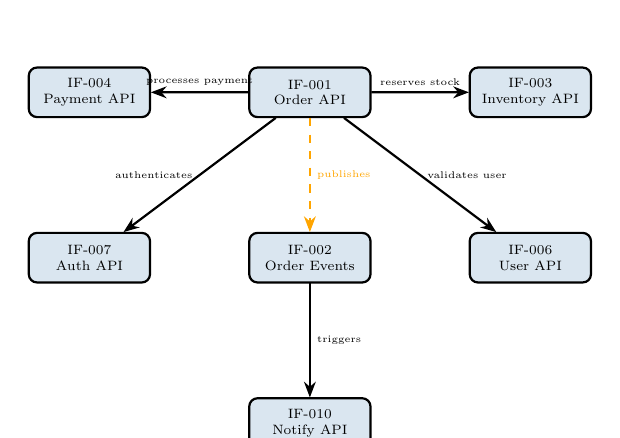
\begin{tikzpicture}[
    scale=0.7,
    transform shape,
    iface/.style={draw, thick, fill=interfacecolor!20, minimum width=2.2cm, minimum height=0.9cm, rounded corners=3pt, font=\scriptsize, align=center},
    uses/.style={-{Stealth[length=2mm]}, thick},
    publishes/.style={-{Stealth[length=2mm]}, thick, dashed, eventcolor}
]
    % Interfaces
    \node[iface] (order) at (0,3) {IF-001\\Order API};
    \node[iface] (events) at (0,0) {IF-002\\Order Events};
    \node[iface] (inv) at (4,3) {IF-003\\Inventory API};
    \node[iface] (pay) at (-4,3) {IF-004\\Payment API};
    \node[iface] (user) at (4,0) {IF-006\\User API};
    \node[iface] (auth) at (-4,0) {IF-007\\Auth API};
    \node[iface] (notify) at (0,-3) {IF-010\\Notify API};
    
    % Dependencies
    \draw[uses] (order) -- node[above, font=\tiny] {reserves stock} (inv);
    \draw[uses] (order) -- node[above, font=\tiny] {processes payment} (pay);
    \draw[uses] (order) -- node[right, font=\tiny] {validates user} (user);
    \draw[publishes] (order) -- node[right, font=\tiny] {publishes} (events);
    \draw[uses] (events) -- node[right, font=\tiny] {triggers} (notify);
    \draw[uses] (order) -- node[left, font=\tiny] {authenticates} (auth);
\end{tikzpicture}
\caption{Interface Dependency Map}
\end{figure}

%==============================================================================
\section{Documentation Conventions}
%==============================================================================

\subsection{Naming Conventions}

\begin{bestpractice}
\textbf{Interface Naming Standards:}

\textbf{Interface IDs:} Use pattern \texttt{IF-NNN} with sequential numbering.

\textbf{API Names:} Use descriptive names indicating domain and purpose (e.g., ``Order Management API'').

\textbf{Endpoints:} Use lowercase, hyphen-separated paths (e.g., \texttt{/order-items}).

\textbf{Operations:} Use verb-noun format for RPC-style (e.g., \texttt{CreateOrder}), noun for resources.

\textbf{Events:} Use past-tense verbs indicating what happened (e.g., \texttt{OrderCreated}).

\textbf{Fields:} Use camelCase for JSON, snake\_case for databases.
\end{bestpractice}

\subsection{Common Data Formats}

\subsubsection{Standard Response Envelope}

\begin{lstlisting}[style=json, caption=Standard API Response Envelope]
{
  "data": { ... },           // Response payload (on success)
  "meta": {
    "requestId": "uuid",     // Correlation ID for tracing
    "timestamp": "ISO8601",  // Response timestamp
    "version": "v1"          // API version
  },
  "pagination": {            // For list responses
    "page": 1,
    "pageSize": 20,
    "totalItems": 150,
    "totalPages": 8
  }
}
\end{lstlisting}

\subsubsection{Standard Error Format}

\begin{lstlisting}[style=json, caption=Standard Error Response]
{
  "error": {
    "code": "VALIDATION_ERROR",    // Machine-readable code
    "message": "Invalid input",    // Human-readable message
    "details": [                   // Detailed field errors
      {
        "field": "email",
        "code": "INVALID_FORMAT",
        "message": "Must be valid email"
      }
    ],
    "requestId": "uuid",           // For support reference
    "documentation": "https://..."  // Link to docs
  }
}
\end{lstlisting}

\subsection{HTTP Status Code Standards}

\begin{longtable}{@{}C{1.5cm} L{3.5cm} L{7.5cm}@{}}
\caption{HTTP Status Code Usage} \\
\toprule
\textbf{Code} & \textbf{Meaning} & \textbf{When to Use} \\
\midrule
\endfirsthead
\toprule
\textbf{Code} & \textbf{Meaning} & \textbf{When to Use} \\
\midrule
\endhead
\bottomrule
\endlastfoot
200 & OK & Successful GET, PUT, PATCH \\
201 & Created & Successful POST creating resource \\
202 & Accepted & Request accepted for async processing \\
204 & No Content & Successful DELETE or PUT with no response body \\
400 & Bad Request & Malformed request syntax or invalid parameters \\
401 & Unauthorized & Missing or invalid authentication \\
403 & Forbidden & Authenticated but not authorized \\
404 & Not Found & Resource does not exist \\
409 & Conflict & Conflict with current state (e.g., duplicate) \\
422 & Unprocessable & Validation error on well-formed request \\
429 & Too Many Requests & Rate limit exceeded \\
500 & Internal Error & Unexpected server error \\
502 & Bad Gateway & Upstream service error \\
503 & Service Unavailable & Temporarily unavailable (maintenance) \\
504 & Gateway Timeout & Upstream service timeout \\
\end{longtable}

\subsection{Authentication Standards}

\begin{longtable}{@{}L{3cm} L{4cm} L{5.5cm}@{}}
\caption{Authentication Methods} \\
\toprule
\textbf{Method} & \textbf{Use Case} & \textbf{Implementation} \\
\midrule
\endfirsthead
\toprule
\textbf{Method} & \textbf{Use Case} & \textbf{Implementation} \\
\midrule
\endhead
\bottomrule
\endlastfoot
Bearer Token (JWT) & User authentication; API access & \texttt{Authorization: Bearer <token>} \\
API Key & Service-to-service; simple clients & \texttt{X-API-Key: <key>} header \\
OAuth 2.0 & Delegated authorization & Authorization code or client credentials flow \\
mTLS & Service mesh; high security & Client certificate validation \\
HMAC Signature & Webhooks; request integrity & \texttt{X-Signature: <hmac>} header \\
\end{longtable}

%==============================================================================
\section{REST API Documentation}
%==============================================================================

\subsection{REST API Specification Template}

This section provides the complete template for documenting REST APIs.

\begin{interfacebox}[IF-001: Order Management API]

\subsection*{A. General Information}

\begin{tabular}{@{}L{3.5cm} L{9cm}@{}}
\textbf{Interface ID:} & IF-001 \\
\textbf{Name:} & Order Management API \\
\textbf{Owning Element:} & Order Service (\texttt{SVC-ORDER-001}) \\
\textbf{Interface Type:} & Provided \\
\textbf{Technology:} & REST over HTTP/1.1, JSON \\
\textbf{Base URL:} & \texttt{https://api.example.com/v1/orders} \\
\textbf{Version:} & v1.3.0 \\
\textbf{Status:} & \statusstable \\
\textbf{OpenAPI Spec:} & \texttt{/specs/order-api-v1.yaml} \\
\end{tabular}

\vspace{0.3cm}
\subsection*{B. Responsibilities and Role}

The Order Management API provides the primary interface for order lifecycle management. It enables clients to create orders, query order status, modify orders before fulfillment, and cancel orders. The API serves as the entry point for all order-related operations in the e-commerce platform.

\textbf{Key Use Cases:}
\begin{itemize}[nosep]
    \item Customer checkout: Create new order from shopping cart
    \item Order tracking: Query order status and history
    \item Order modification: Update shipping address before shipment
    \item Order cancellation: Cancel order with refund initiation
    \item Admin operations: List and search orders for support
\end{itemize}

\textbf{Stakeholders:}
\begin{itemize}[nosep]
    \item Web/Mobile frontend teams
    \item Customer service applications
    \item Partner integration systems
    \item Analytics and reporting systems
\end{itemize}

\vspace{0.3cm}
\subsection*{C. Operations}

\begin{longtable}{@{}L{0.8cm} L{3.5cm} L{8cm}@{}}
\toprule
\textbf{} & \textbf{Endpoint} & \textbf{Description} \\
\midrule
\httppost & \texttt{/orders} & Create a new order \\
\httpget & \texttt{/orders} & List orders with filtering and pagination \\
\httpget & \texttt{/orders/\{id\}} & Get order details by ID \\
\httppatch & \texttt{/orders/\{id\}} & Update order (limited fields) \\
\httpdelete & \texttt{/orders/\{id\}} & Cancel order \\
\httpget & \texttt{/orders/\{id\}/items} & Get order line items \\
\httppost & \texttt{/orders/\{id\}/items} & Add item to order (draft only) \\
\httpget & \texttt{/orders/\{id\}/history} & Get order status history \\
\httppost & \texttt{/orders/\{id\}/actions/confirm} & Confirm pending order \\
\httppost & \texttt{/orders/\{id\}/actions/ship} & Mark order as shipped \\
\bottomrule
\end{longtable}

\vspace{0.3cm}
\subsection*{D. Operation Details}

\subsubsection*{POST /orders -- Create Order}

\textbf{Description:} Creates a new order from the provided items, customer, and shipping information.

\textbf{Request Body:}
\begin{lstlisting}[style=json]
{
  "customerId": "cust_123abc",
  "items": [
    {
      "productId": "prod_456def",
      "quantity": 2,
      "priceOverride": null
    }
  ],
  "shippingAddress": {
    "street": "123 Main St",
    "city": "Seattle",
    "state": "WA",
    "postalCode": "98101",
    "country": "US"
  },
  "billingAddress": { ... },
  "paymentMethodId": "pm_789ghi",
  "couponCode": "SAVE10",
  "metadata": {
    "source": "web",
    "campaign": "summer-sale"
  }
}
\end{lstlisting}

\textbf{Response (201 Created):}
\begin{lstlisting}[style=json]
{
  "data": {
    "id": "ord_abc123",
    "status": "pending_payment",
    "customerId": "cust_123abc",
    "items": [...],
    "subtotal": 9999,
    "tax": 875,
    "shipping": 599,
    "discount": -1000,
    "total": 10473,
    "currency": "USD",
    "createdAt": "2024-01-15T10:30:00Z",
    "estimatedDelivery": "2024-01-20"
  },
  "meta": {
    "requestId": "req_xyz789"
  }
}
\end{lstlisting}

\textbf{Validation Rules:}
\begin{itemize}[nosep]
    \item \texttt{customerId}: Required; must exist and be active
    \item \texttt{items}: Required; 1-100 items allowed
    \item \texttt{items[].quantity}: Required; 1-999
    \item \texttt{shippingAddress}: Required for physical goods
    \item \texttt{paymentMethodId}: Required; must belong to customer
\end{itemize}

\textbf{Error Responses:}
\begin{itemize}[nosep]
    \item \texttt{400}: Invalid request format
    \item \texttt{401}: Authentication required
    \item \texttt{403}: Customer cannot place orders
    \item \texttt{422}: Validation failed (see details)
    \item \texttt{409}: Insufficient inventory
\end{itemize}

\subsubsection*{GET /orders -- List Orders}

\textbf{Description:} Returns a paginated list of orders matching the query criteria.

\textbf{Query Parameters:}

\begin{tabular}{@{}L{3cm} L{2cm} L{2cm} L{5.2cm}@{}}
\toprule
\textbf{Parameter} & \textbf{Type} & \textbf{Required} & \textbf{Description} \\
\midrule
\texttt{customerId} & string & No & Filter by customer \\
\texttt{status} & string[] & No & Filter by status(es) \\
\texttt{createdAfter} & datetime & No & Orders after date \\
\texttt{createdBefore} & datetime & No & Orders before date \\
\texttt{page} & integer & No & Page number (default: 1) \\
\texttt{pageSize} & integer & No & Items per page (default: 20, max: 100) \\
\texttt{sort} & string & No & Sort field (default: -createdAt) \\
\bottomrule
\end{tabular}

\textbf{Example Request:}
\begin{lstlisting}[style=http]
GET /v1/orders?customerId=cust_123&status=pending,confirmed&pageSize=10
Authorization: Bearer eyJhbG...
\end{lstlisting}

\vspace{0.3cm}
\subsection*{E. Data Types}

\subsubsection*{Order Object}

\begin{tabular}{@{}L{3cm} L{2cm} L{2cm} L{5.2cm}@{}}
\toprule
\textbf{Field} & \textbf{Type} & \textbf{Required} & \textbf{Description} \\
\midrule
\texttt{id} & string & Yes & Unique order identifier \\
\texttt{status} & enum & Yes & Current order status \\
\texttt{customerId} & string & Yes & Customer reference \\
\texttt{items} & OrderItem[] & Yes & Line items \\
\texttt{subtotal} & integer & Yes & Subtotal in cents \\
\texttt{tax} & integer & Yes & Tax amount in cents \\
\texttt{shipping} & integer & Yes & Shipping cost in cents \\
\texttt{discount} & integer & No & Discount in cents (negative) \\
\texttt{total} & integer & Yes & Total in cents \\
\texttt{currency} & string & Yes & ISO 4217 currency code \\
\texttt{shippingAddress} & Address & Yes & Delivery address \\
\texttt{billingAddress} & Address & No & Billing address \\
\texttt{createdAt} & datetime & Yes & Creation timestamp \\
\texttt{updatedAt} & datetime & Yes & Last update timestamp \\
\texttt{metadata} & object & No & Custom key-value pairs \\
\bottomrule
\end{tabular}

\subsubsection*{Order Status Enum}

\begin{tabular}{@{}L{3.5cm} L{9cm}@{}}
\toprule
\textbf{Value} & \textbf{Description} \\
\midrule
\texttt{draft} & Order being composed; not yet submitted \\
\texttt{pending\_payment} & Submitted; awaiting payment confirmation \\
\texttt{confirmed} & Payment received; awaiting fulfillment \\
\texttt{processing} & Being prepared for shipment \\
\texttt{shipped} & Handed to carrier \\
\texttt{delivered} & Confirmed delivered \\
\texttt{cancelled} & Cancelled by customer or system \\
\texttt{refunded} & Refund processed \\
\bottomrule
\end{tabular}

\vspace{0.3cm}
\subsection*{F. Protocol Details}

\textbf{Transport:} HTTPS (TLS 1.2+) required; HTTP redirects to HTTPS

\textbf{Content Type:} \texttt{application/json} for request and response bodies

\textbf{Character Encoding:} UTF-8

\textbf{Date Format:} ISO 8601 (\texttt{2024-01-15T10:30:00Z})

\textbf{Monetary Values:} Integer cents (e.g., \$99.99 = 9999)

\textbf{Compression:} gzip supported via \texttt{Accept-Encoding}

\textbf{CORS:} Enabled for approved origins; credentials allowed

\vspace{0.3cm}
\subsection*{G. Semantics and Behavior}

\textbf{Idempotency:}
\begin{itemize}[nosep]
    \item GET, PUT, DELETE are idempotent
    \item POST /orders supports idempotency via \texttt{Idempotency-Key} header
    \item Duplicate requests within 24h return original response
\end{itemize}

\textbf{Concurrency Control:}
\begin{itemize}[nosep]
    \item Optimistic locking via \texttt{ETag} / \texttt{If-Match} headers
    \item PATCH/DELETE without \texttt{If-Match} may conflict
    \item 409 Conflict returned on version mismatch
\end{itemize}

\textbf{State Transitions:}
\begin{itemize}[nosep]
    \item Orders follow defined state machine (see Order Status)
    \item Invalid transitions return 422 with allowed transitions
    \item Some transitions trigger downstream events
\end{itemize}

\vspace{0.3cm}
\subsection*{H. Error Handling}

\textbf{Error Codes:}

\begin{tabular}{@{}L{4cm} L{8.5cm}@{}}
\toprule
\textbf{Code} & \textbf{Description} \\
\midrule
\texttt{VALIDATION\_ERROR} & Request validation failed \\
\texttt{RESOURCE\_NOT\_FOUND} & Order ID does not exist \\
\texttt{INVALID\_STATE\_TRANSITION} & Operation not allowed in current state \\
\texttt{INSUFFICIENT\_INVENTORY} & Not enough stock for order \\
\texttt{PAYMENT\_FAILED} & Payment could not be processed \\
\texttt{RATE\_LIMIT\_EXCEEDED} & Too many requests \\
\texttt{INTERNAL\_ERROR} & Unexpected server error \\
\bottomrule
\end{tabular}

\textbf{Retry Policy:}
\begin{itemize}[nosep]
    \item 429: Retry after \texttt{Retry-After} header value
    \item 503: Retry with exponential backoff (initial 1s, max 60s)
    \item 5xx: Retry up to 3 times with jitter
    \item 4xx (except 429): Do not retry; fix request
\end{itemize}

\vspace{0.3cm}
\subsection*{I. Quality of Service}

\begin{tabular}{@{}L{4cm} L{3cm} L{5.5cm}@{}}
\toprule
\textbf{Metric} & \textbf{Target} & \textbf{Notes} \\
\midrule
Response Time (p50) & $<$ 100ms & Typical operations \\
Response Time (p95) & $<$ 500ms & Under normal load \\
Response Time (p99) & $<$ 2000ms & Peak conditions \\
Availability & 99.95\% & Monthly uptime \\
Throughput & 1000 req/s & Per API instance \\
Rate Limit (standard) & 100 req/min & Per API key \\
Rate Limit (premium) & 1000 req/min & Enterprise tier \\
\bottomrule
\end{tabular}

\vspace{0.3cm}
\subsection*{J. Security}

\textbf{Authentication:} Bearer token (JWT) required for all endpoints

\textbf{Authorization:}
\begin{itemize}[nosep]
    \item Customers: Access own orders only
    \item Admins: Access all orders with \texttt{orders:admin} scope
    \item Services: Access via service account with \texttt{orders:service} scope
\end{itemize}

\textbf{Required Scopes:}

\begin{tabular}{@{}L{4cm} L{8.5cm}@{}}
\toprule
\textbf{Scope} & \textbf{Permissions} \\
\midrule
\texttt{orders:read} & GET operations \\
\texttt{orders:write} & POST, PATCH, DELETE operations \\
\texttt{orders:admin} & All operations; all orders \\
\bottomrule
\end{tabular}

\textbf{Data Protection:}
\begin{itemize}[nosep]
    \item PII fields encrypted at rest
    \item TLS 1.2+ required in transit
    \item Audit logging for all mutations
\end{itemize}

\vspace{0.3cm}
\subsection*{K. Dependencies}

\begin{tabular}{@{}L{3cm} L{3cm} L{6.5cm}@{}}
\toprule
\textbf{Interface} & \textbf{Purpose} & \textbf{Failure Impact} \\
\midrule
IF-003 (Inventory) & Stock reservation & Order creation fails \\
IF-004 (Payment) & Payment processing & Order stuck in pending \\
IF-006 (User) & Customer validation & Order creation fails \\
IF-010 (Notification) & Email/SMS alerts & Degraded (order succeeds) \\
\bottomrule
\end{tabular}

\vspace{0.3cm}
\subsection*{L. Versioning}

\textbf{Version Strategy:} URL path versioning (\texttt{/v1/}, \texttt{/v2/})

\textbf{Current Versions:}
\begin{itemize}[nosep]
    \item \texttt{v1}: Current stable version (this document)
    \item \texttt{v2}: Beta; new order model (separate doc)
\end{itemize}

\textbf{Deprecation Policy:}
\begin{itemize}[nosep]
    \item 12 months notice before version sunset
    \item \texttt{Deprecation} header added to responses
    \item Migration guide provided
\end{itemize}

\textbf{Breaking Changes (require new version):}
\begin{itemize}[nosep]
    \item Removing endpoints or fields
    \item Changing field types
    \item Changing error codes
    \item Changing authentication
\end{itemize}

\textbf{Non-Breaking Changes (same version):}
\begin{itemize}[nosep]
    \item Adding optional fields
    \item Adding new endpoints
    \item Adding new enum values
    \item Relaxing validation
\end{itemize}

\vspace{0.3cm}
\subsection*{M. Usage Examples}

\textbf{Create Order (cURL):}
\begin{lstlisting}[language=bash]
curl -X POST https://api.example.com/v1/orders \
  -H "Authorization: Bearer eyJhbG..." \
  -H "Content-Type: application/json" \
  -H "Idempotency-Key: unique-request-id" \
  -d '{
    "customerId": "cust_123abc",
    "items": [{"productId": "prod_456", "quantity": 2}],
    "shippingAddress": {...},
    "paymentMethodId": "pm_789"
  }'
\end{lstlisting}

\textbf{List Orders with Filtering:}
\begin{lstlisting}[language=bash]
curl "https://api.example.com/v1/orders?status=pending&page=1" \
  -H "Authorization: Bearer eyJhbG..."
\end{lstlisting}

\vspace{0.3cm}
\subsection*{N. Traceability}

\textbf{Requirements:}
\begin{itemize}[nosep]
    \item REQ-FUNC-001: Order creation
    \item REQ-FUNC-002: Order tracking
    \item REQ-FUNC-003: Order cancellation
    \item REQ-NFR-001: $<$500ms response time
\end{itemize}

\textbf{Architectural Decisions:}
\begin{itemize}[nosep]
    \item ADR-005: REST for synchronous APIs
    \item ADR-012: JWT authentication
    \item ADR-015: Idempotency key pattern
\end{itemize}

\textbf{Test Contracts:} \texttt{/tests/contracts/order-api.pact}

\vspace{0.3cm}
\subsection*{O. Change History}

\begin{tabular}{@{}L{1.2cm} L{2cm} L{2.2cm} L{6.8cm}@{}}
\toprule
\textbf{Ver} & \textbf{Date} & \textbf{Author} & \textbf{Changes} \\
\midrule
1.0.0 & 2023-06-01 & J. Smith & Initial release \\
1.1.0 & 2023-09-15 & A. Jones & Added order actions endpoints \\
1.2.0 & 2024-01-10 & J. Smith & Added metadata field \\
1.3.0 & 2024-03-01 & B. Wilson & Added pagination to list endpoint \\
\bottomrule
\end{tabular}
\end{interfacebox}

%==============================================================================
\section{Event Interface Documentation}
%==============================================================================

\subsection{Event Interface Specification Template}

\begin{eventbox}[IF-002: Order Events]

\subsection*{A. General Information}

\begin{tabular}{@{}L{3.5cm} L{9cm}@{}}
\textbf{Interface ID:} & IF-002 \\
\textbf{Name:} & Order Events \\
\textbf{Owning Element:} & Order Service (\texttt{SVC-ORDER-001}) \\
\textbf{Interface Type:} & Provided (Publisher) \\
\textbf{Technology:} & Apache Kafka \\
\textbf{Topic:} & \texttt{orders.events.v1} \\
\textbf{Version:} & v1.2.0 \\
\textbf{Status:} & \statusstable \\
\textbf{AsyncAPI Spec:} & \texttt{/specs/order-events-v1.yaml} \\
\end{tabular}

\vspace{0.3cm}
\subsection*{B. Responsibilities and Role}

The Order Events interface publishes domain events for all significant order state changes. It enables downstream services to react to order lifecycle events without tight coupling to the Order Service.

\textbf{Key Use Cases:}
\begin{itemize}[nosep]
    \item Inventory: Release reservations on cancellation
    \item Payments: Initiate refunds on cancellation
    \item Notifications: Send customer communications
    \item Analytics: Track order funnel metrics
    \item Search: Update order search index
\end{itemize}

\vspace{0.3cm}
\subsection*{C. Event Types}

\begin{longtable}{@{}L{3.5cm} L{4cm} L{5cm}@{}}
\toprule
\textbf{Event Type} & \textbf{Trigger} & \textbf{Key Data} \\
\midrule
\texttt{OrderCreated} & New order submitted & Full order details \\
\texttt{OrderConfirmed} & Payment successful & Order ID, confirmation time \\
\texttt{OrderUpdated} & Order modified & Changed fields, version \\
\texttt{OrderShipped} & Shipment created & Tracking number, carrier \\
\texttt{OrderDelivered} & Delivery confirmed & Delivery timestamp \\
\texttt{OrderCancelled} & Order cancelled & Cancellation reason \\
\texttt{OrderRefunded} & Refund processed & Refund amount, method \\
\bottomrule
\end{longtable}

\vspace{0.3cm}
\subsection*{D. Event Schema}

\subsubsection*{Event Envelope}

\begin{lstlisting}[style=json]
{
  "eventId": "evt_abc123xyz",
  "eventType": "OrderCreated",
  "eventVersion": "1.0",
  "timestamp": "2024-01-15T10:30:00.123Z",
  "source": "order-service",
  "correlationId": "req_xyz789",
  "partitionKey": "ord_def456",
  "data": { ... }
}
\end{lstlisting}

\subsubsection*{OrderCreated Event Data}

\begin{lstlisting}[style=json]
{
  "orderId": "ord_def456",
  "customerId": "cust_123abc",
  "status": "pending_payment",
  "items": [
    {
      "productId": "prod_789",
      "sku": "WIDGET-001",
      "quantity": 2,
      "unitPrice": 4999,
      "totalPrice": 9998
    }
  ],
  "subtotal": 9998,
  "tax": 850,
  "shipping": 599,
  "total": 11447,
  "currency": "USD",
  "shippingAddress": { ... },
  "createdAt": "2024-01-15T10:30:00Z"
}
\end{lstlisting}

\subsubsection*{OrderCancelled Event Data}

\begin{lstlisting}[style=json]
{
  "orderId": "ord_def456",
  "customerId": "cust_123abc",
  "previousStatus": "confirmed",
  "reason": "customer_request",
  "reasonDetails": "Changed mind",
  "cancelledBy": "customer",
  "cancelledAt": "2024-01-15T14:00:00Z",
  "refundInitiated": true,
  "refundAmount": 11447
}
\end{lstlisting}

\vspace{0.3cm}
\subsection*{E. Protocol and Transport}

\textbf{Broker:} Apache Kafka 3.x

\textbf{Topic Configuration:}
\begin{itemize}[nosep]
    \item Partitions: 12
    \item Replication Factor: 3
    \item Retention: 7 days
    \item Cleanup Policy: delete
\end{itemize}

\textbf{Serialization:}
\begin{itemize}[nosep]
    \item Format: JSON
    \item Schema Registry: Confluent Schema Registry
    \item Compatibility: BACKWARD
\end{itemize}

\textbf{Partitioning:}
\begin{itemize}[nosep]
    \item Key: \texttt{orderId}
    \item Guarantees per-order ordering
\end{itemize}

\vspace{0.3cm}
\subsection*{F. Delivery Semantics}

\textbf{Delivery Guarantee:} At-least-once

\textbf{Ordering:} Per partition (same order ID = same partition)

\textbf{Idempotency:}
\begin{itemize}[nosep]
    \item \texttt{eventId} is globally unique
    \item Consumers must handle duplicates
    \item Recommended: Track processed eventIds
\end{itemize}

\textbf{Consumer Groups:}
\begin{itemize}[nosep]
    \item Each service uses unique group ID
    \item Enables independent consumption
    \item Example: \texttt{inventory-service-orders}
\end{itemize}

\vspace{0.3cm}
\subsection*{G. Error Handling}

\textbf{Dead Letter Topic:} \texttt{orders.events.v1.dlq}

\textbf{Poison Message Handling:}
\begin{itemize}[nosep]
    \item Messages failing 3x sent to DLQ
    \item Include original message + error details
    \item Alert on DLQ growth
\end{itemize}

\textbf{Consumer Failure Recovery:}
\begin{itemize}[nosep]
    \item Committed offsets preserved
    \item Resume from last commit on restart
    \item Replay from timestamp if needed
\end{itemize}

\vspace{0.3cm}
\subsection*{H. Quality of Service}

\begin{tabular}{@{}L{4cm} L{3cm} L{5.5cm}@{}}
\toprule
\textbf{Metric} & \textbf{Target} & \textbf{Notes} \\
\midrule
Publish Latency (p99) & $<$ 100ms & From commit to broker ack \\
End-to-End Latency & $<$ 5s & Typical consumer processing \\
Availability & 99.9\% & Kafka cluster uptime \\
Throughput & 10,000 msg/s & Peak sustained \\
Consumer Lag & $<$ 1000 msgs & Alert threshold \\
\bottomrule
\end{tabular}

\vspace{0.3cm}
\subsection*{I. Consumer Guidelines}

\begin{lstlisting}[language=java, caption=Consumer Implementation Example]
@KafkaListener(topics = "orders.events.v1", 
               groupId = "notification-service")
public void handleOrderEvent(OrderEvent event) {
    // Idempotency check
    if (processedEvents.contains(event.getEventId())) {
        log.info("Duplicate event ignored: {}", event.getEventId());
        return;
    }
    
    switch (event.getEventType()) {
        case "OrderCreated":
            sendOrderConfirmationEmail(event.getData());
            break;
        case "OrderShipped":
            sendShippingNotification(event.getData());
            break;
        case "OrderCancelled":
            sendCancellationEmail(event.getData());
            break;
    }
    
    processedEvents.add(event.getEventId());
}
\end{lstlisting}

\vspace{0.3cm}
\subsection*{J. Schema Evolution}

\textbf{Compatibility Mode:} BACKWARD (new schema can read old data)

\textbf{Evolution Rules:}
\begin{itemize}[nosep]
    \item Adding optional fields: Allowed
    \item Removing fields: Requires new version
    \item Changing field types: Requires new version
    \item Renaming fields: Requires new version
\end{itemize}

\textbf{Version History:}
\begin{itemize}[nosep]
    \item v1.0: Initial schema
    \item v1.1: Added \texttt{refundInitiated} to cancellation
    \item v1.2: Added \texttt{correlationId} to envelope
\end{itemize}

\end{eventbox}

%==============================================================================
\section{gRPC Interface Documentation}
%==============================================================================

\subsection{gRPC Service Specification}

\begin{interfacebox}[IF-003: Inventory Service (gRPC)]

\subsection*{A. General Information}

\begin{tabular}{@{}L{3.5cm} L{9cm}@{}}
\textbf{Interface ID:} & IF-003 \\
\textbf{Name:} & Inventory Service \\
\textbf{Owning Element:} & Inventory Service (\texttt{SVC-INV-001}) \\
\textbf{Interface Type:} & Provided \\
\textbf{Technology:} & gRPC over HTTP/2 \\
\textbf{Proto Package:} & \texttt{com.example.inventory.v1} \\
\textbf{Proto File:} & \texttt{/protos/inventory/v1/inventory.proto} \\
\textbf{Version:} & v1 \\
\textbf{Status:} & \statusstable \\
\end{tabular}

\vspace{0.3cm}
\subsection*{B. Service Definition}

\begin{lstlisting}[language=C, caption=inventory.proto]
syntax = "proto3";

package com.example.inventory.v1;

service InventoryService {
  // Check stock availability for products
  rpc CheckAvailability(CheckAvailabilityRequest) 
      returns (CheckAvailabilityResponse);
  
  // Reserve stock for an order
  rpc ReserveStock(ReserveStockRequest) 
      returns (ReserveStockResponse);
  
  // Release previously reserved stock
  rpc ReleaseReservation(ReleaseReservationRequest) 
      returns (ReleaseReservationResponse);
  
  // Commit reservation (deduct from inventory)
  rpc CommitReservation(CommitReservationRequest) 
      returns (CommitReservationResponse);
  
  // Stream inventory updates
  rpc WatchInventory(WatchInventoryRequest) 
      returns (stream InventoryUpdate);
}
\end{lstlisting}

\vspace{0.3cm}
\subsection*{C. Message Types}

\begin{lstlisting}[language=C]
message CheckAvailabilityRequest {
  repeated string product_ids = 1;
  string warehouse_id = 2;  // Optional; all warehouses if empty
}

message CheckAvailabilityResponse {
  repeated ProductAvailability availability = 1;
}

message ProductAvailability {
  string product_id = 1;
  int32 available_quantity = 2;
  int32 reserved_quantity = 3;
  repeated WarehouseStock warehouse_breakdown = 4;
}

message ReserveStockRequest {
  string order_id = 1;
  repeated ReservationItem items = 2;
  int32 ttl_seconds = 3;  // Reservation expiry (default: 900)
}

message ReservationItem {
  string product_id = 1;
  int32 quantity = 2;
  string warehouse_id = 3;  // Optional
}

message ReserveStockResponse {
  string reservation_id = 1;
  ReservationStatus status = 2;
  repeated ReservationResult items = 3;
  google.protobuf.Timestamp expires_at = 4;
}

enum ReservationStatus {
  RESERVATION_STATUS_UNSPECIFIED = 0;
  RESERVATION_STATUS_SUCCESS = 1;
  RESERVATION_STATUS_PARTIAL = 2;
  RESERVATION_STATUS_FAILED = 3;
}
\end{lstlisting}

\vspace{0.3cm}
\subsection*{D. Error Handling}

\textbf{gRPC Status Codes:}

\begin{tabular}{@{}L{3.5cm} L{9cm}@{}}
\toprule
\textbf{Code} & \textbf{When Used} \\
\midrule
\texttt{OK} & Success \\
\texttt{INVALID\_ARGUMENT} & Invalid product ID, negative quantity \\
\texttt{NOT\_FOUND} & Product or reservation not found \\
\texttt{FAILED\_PRECONDITION} & Insufficient stock for reservation \\
\texttt{ALREADY\_EXISTS} & Duplicate reservation ID \\
\texttt{RESOURCE\_EXHAUSTED} & Rate limit exceeded \\
\texttt{UNAVAILABLE} & Service temporarily unavailable \\
\texttt{DEADLINE\_EXCEEDED} & Request timeout \\
\bottomrule
\end{tabular}

\textbf{Error Details:}
\begin{lstlisting}[language=C]
message InsufficientStockError {
  string product_id = 1;
  int32 requested = 2;
  int32 available = 3;
}
\end{lstlisting}

\vspace{0.3cm}
\subsection*{E. Quality of Service}

\begin{tabular}{@{}L{4cm} L{3cm} L{5.5cm}@{}}
\toprule
\textbf{Metric} & \textbf{Target} & \textbf{Notes} \\
\midrule
Latency (p50) & $<$ 10ms & Unary calls \\
Latency (p99) & $<$ 100ms & Under load \\
Throughput & 5000 req/s & Per instance \\
\bottomrule
\end{tabular}

\textbf{Deadlines:} Clients should set 5s deadline for unary calls.

\textbf{Retry Policy:}
\begin{lstlisting}[style=json]
{
  "methodConfig": [{
    "name": [{"service": "inventory.v1.InventoryService"}],
    "retryPolicy": {
      "maxAttempts": 3,
      "initialBackoff": "0.1s",
      "maxBackoff": "1s",
      "backoffMultiplier": 2,
      "retryableStatusCodes": ["UNAVAILABLE", "DEADLINE_EXCEEDED"]
    }
  }]
}
\end{lstlisting}

\vspace{0.3cm}
\subsection*{F. Authentication}

\textbf{Method:} mTLS (mutual TLS) for service-to-service

\textbf{Metadata Headers:}
\begin{itemize}[nosep]
    \item \texttt{x-request-id}: Correlation ID for tracing
    \item \texttt{x-caller-service}: Calling service name
\end{itemize}

\end{interfacebox}

%==============================================================================
\section{Webhook Interface Documentation}
%==============================================================================

\begin{interfacebox}[IF-005: Payment Webhooks]

\subsection*{A. General Information}

\begin{tabular}{@{}L{3.5cm} L{9cm}@{}}
\textbf{Interface ID:} & IF-005 \\
\textbf{Name:} & Payment Webhooks \\
\textbf{Owning Element:} & Payment Service (\texttt{SVC-PAY-001}) \\
\textbf{Interface Type:} & Provided (Outbound) \\
\textbf{Technology:} & HTTP POST callbacks \\
\textbf{Version:} & v1 \\
\textbf{Status:} & \statusstable \\
\end{tabular}

\vspace{0.3cm}
\subsection*{B. Webhook Events}

\begin{tabular}{@{}L{3.5cm} L{9cm}@{}}
\toprule
\textbf{Event Type} & \textbf{Description} \\
\midrule
\texttt{payment.succeeded} & Payment successfully captured \\
\texttt{payment.failed} & Payment attempt failed \\
\texttt{payment.refunded} & Refund processed \\
\texttt{payment.disputed} & Chargeback initiated \\
\bottomrule
\end{tabular}

\vspace{0.3cm}
\subsection*{C. Webhook Payload}

\begin{lstlisting}[style=json]
{
  "id": "whk_evt_abc123",
  "type": "payment.succeeded",
  "created": "2024-01-15T10:30:00Z",
  "data": {
    "paymentId": "pay_xyz789",
    "orderId": "ord_def456",
    "amount": 11447,
    "currency": "USD",
    "status": "succeeded",
    "paymentMethod": {
      "type": "card",
      "last4": "4242",
      "brand": "visa"
    }
  }
}
\end{lstlisting}

\vspace{0.3cm}
\subsection*{D. Signature Verification}

All webhooks include HMAC signature for verification:

\begin{lstlisting}[language=bash]
# Headers sent with webhook
X-Webhook-Signature: sha256=abc123...
X-Webhook-Timestamp: 1705315800
X-Webhook-Id: whk_evt_abc123
\end{lstlisting}

\textbf{Verification Steps:}
\begin{enumerate}[nosep]
    \item Extract timestamp and signature from headers
    \item Reject if timestamp $>$ 5 minutes old (replay protection)
    \item Compute expected signature: \texttt{HMAC-SHA256(timestamp.payload, secret)}
    \item Compare signatures using constant-time comparison
\end{enumerate}

\vspace{0.3cm}
\subsection*{E. Delivery Behavior}

\textbf{Retry Schedule:} 1min, 5min, 30min, 2hr, 24hr (5 attempts)

\textbf{Success Response:} 2xx status code

\textbf{Failure Response:} Any non-2xx triggers retry

\textbf{Timeout:} 30 seconds per attempt

\textbf{Idempotency:} Use \texttt{X-Webhook-Id} to detect duplicates

\end{interfacebox}

%==============================================================================
\section{Interface Governance}
%==============================================================================

\subsection{Interface Lifecycle}

\begin{figure}[H]
\centering
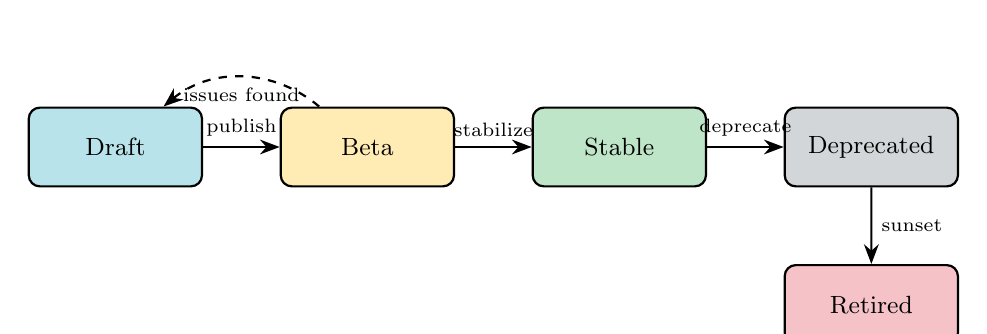
\begin{tikzpicture}[
    scale=0.8,
    state/.style={draw, thick, rounded corners, minimum width=2.2cm, minimum height=1cm, font=\small},
    arrow/.style={-{Stealth[length=2.5mm]}, thick}
]
    \node[state, fill=infoblue!30] (draft) at (0,0) {Draft};
    \node[state, fill=betacolor!30] (beta) at (4,0) {Beta};
    \node[state, fill=stablecolor!30] (stable) at (8,0) {Stable};
    \node[state, fill=deprecatedcolor!30] (dep) at (12,0) {Deprecated};
    \node[state, fill=errorcolor!30] (retired) at (12,-2.5) {Retired};
    
    \draw[arrow] (draft) -- node[above, font=\scriptsize] {publish} (beta);
    \draw[arrow] (beta) -- node[above, font=\scriptsize] {stabilize} (stable);
    \draw[arrow] (stable) -- node[above, font=\scriptsize] {deprecate} (dep);
    \draw[arrow] (dep) -- node[right, font=\scriptsize] {sunset} (retired);
    \draw[arrow, dashed] (beta) to[bend right=40] node[below, font=\scriptsize] {issues found} (draft);
\end{tikzpicture}
\caption{Interface Lifecycle States}
\end{figure}

\subsection{Breaking Change Policy}

\begin{warning}
\textbf{Breaking Changes Require:}
\begin{itemize}[nosep]
    \item New major version (v1 $\rightarrow$ v2)
    \item 12 months deprecation notice for public APIs
    \item 6 months for internal APIs
    \item Migration guide documentation
    \item Consumer notification
\end{itemize}
\end{warning}

\subsection{Interface Review Checklist}

\begin{itemize}[leftmargin=2cm]
    \item[$\square$] All operations documented with request/response schemas
    \item[$\square$] Error codes and handling documented
    \item[$\square$] Authentication and authorization specified
    \item[$\square$] Rate limits and quotas defined
    \item[$\square$] Versioning strategy documented
    \item[$\square$] Examples provided for all operations
    \item[$\square$] Machine-readable spec (OpenAPI/AsyncAPI) available
    \item[$\square$] Contract tests implemented
    \item[$\square$] Traceability to requirements established
\end{itemize}

%==============================================================================
\section{Appendix A: OpenAPI Template}
%==============================================================================

\begin{lstlisting}[language=yaml, caption=OpenAPI Template (openapi.yaml)]
openapi: 3.1.0
info:
  title: Service Name API
  version: 1.0.0
  description: |
    Detailed description of the API.
  contact:
    name: API Support
    email: api-support@example.com

servers:
  - url: https://api.example.com/v1
    description: Production

security:
  - bearerAuth: []

paths:
  /resources:
    get:
      summary: List resources
      operationId: listResources
      tags: [Resources]
      parameters:
        - name: page
          in: query
          schema:
            type: integer
            default: 1
      responses:
        '200':
          description: Success
          content:
            application/json:
              schema:
                $ref: '#/components/schemas/ResourceList'

components:
  securitySchemes:
    bearerAuth:
      type: http
      scheme: bearer
      bearerFormat: JWT
  schemas:
    ResourceList:
      type: object
      properties:
        data:
          type: array
          items:
            $ref: '#/components/schemas/Resource'
\end{lstlisting}

%==============================================================================
\section{Appendix B: Glossary}
%==============================================================================

\begin{description}[leftmargin=3cm, style=nextline]
    \item[API] Application Programming Interface; contract for programmatic interaction
    \item[AsyncAPI] Specification for documenting event-driven APIs
    \item[Endpoint] A specific URL path that accepts requests
    \item[gRPC] Google Remote Procedure Call; high-performance RPC framework
    \item[Idempotency] Property where multiple identical requests have same effect as one
    \item[OpenAPI] Specification for documenting REST APIs (formerly Swagger)
    \item[Payload] The data content of a request or response
    \item[Protocol] Rules governing communication between systems
    \item[Rate Limit] Maximum number of requests allowed per time period
    \item[Schema] Definition of data structure and types
    \item[Webhook] HTTP callback triggered by an event
\end{description}

%==============================================================================
\section{Appendix C: References}
%==============================================================================

\begin{enumerate}
    \item OpenAPI Initiative. (2023). \textit{OpenAPI Specification 3.1}. \url{https://spec.openapis.org}
    
    \item AsyncAPI Initiative. (2023). \textit{AsyncAPI Specification 2.6}. \url{https://www.asyncapi.com}
    
    \item Google. (2023). \textit{API Design Guide}. \url{https://cloud.google.com/apis/design}
    
    \item Masse, M. (2011). \textit{REST API Design Rulebook}. O'Reilly Media.
    
    \item Clements, P., et al. (2010). \textit{Documenting Software Architectures}. Addison-Wesley.
    
    \item Lauret, A. (2019). \textit{The Design of Web APIs}. Manning Publications.
    
    \item gRPC Authors. (2023). \textit{gRPC Documentation}. \url{https://grpc.io/docs}
    
    \item Fielding, R. (2000). ``Architectural Styles and the Design of Network-based Software Architectures.'' Doctoral dissertation, UC Irvine.
\end{enumerate}

\end{document}